\documentclass[a4paper]{article}


\usepackage[margin=1.5in]{geometry}
\usepackage{color}
\usepackage{url}
\usepackage[utf8]{inputenc} % make weird characters work
\usepackage{graphicx}

\usepackage[english,serbian]{babel}
%\usepackage[english,serbianc]{babel} %ukljuciti babel sa ovim opcijama, umesto gornjim, ukoliko se koristi cirilica
\setcounter{tocdepth}{3}
\usepackage[unicode]{hyperref}
\hypersetup{colorlinks,citecolor=green,filecolor=green,linkcolor=blue,urlcolor=blue}
\usepackage{amsmath}
\usepackage{amssymb}
\usepackage[linesnumbered,ruled]{algorithm2e}

\begin{document}

\title{Napadi na supersingularne kriptografske sisteme umetanjem greške\\ \small{~\\Seminarski rad u okviru kursa Kriptografija\\ Prof. Miodrag Živković\\Matematički fakultet}}

\author{Bukurov Anja 1082/2016}
\date{27.~maj 2017.}
\maketitle

\abstract{
Predstavljamo prvi napad umetanjem greške na kripto sisteme koji su zasnovani na supersingularnim izogenijima. Tokom računanja pomoćnih tačaka, napad cilja da promeni početnu tačku nekom slučajno odabranom tačkom na krivoj umetanjem greške. Pokazaćemo da će ovakav napad otkriti tajnu izogeniju jednom uspešnom smetnjom koja ima visoku verovatnoću uspeha.}

\tableofcontents

\newpage

\section{Uvod}

Kriptografske sisteme zasnovane na izogenijama između supersingularnih eliptičkih krivih predložili su Jao i De Feo 2011. godine kao kandidat za kriptografski protokol. Umesto da se oslanja na problem diskretnog logaritma, koji je osetljiv na Šorov (engl. Shor) algoritam, ovaj protokol zasnovan je na problemu pronalaženja izogenija između supersingularnih eliptičkih krivih.

Napad umetanjem greške iskorišćava curenje osetljivih informacija kada implementacija radi pod neočekivanim uslovima. U ovom radu ispitujemo efekte promene tačke $P$ u neko slučajno odabranu tačku $P_0$ i pokušaj da se otkrije tajna, a to je u ovom slučaju izogenija $\phi$. Napad bi bio u mogućnosti da otkrije celu tajnu $\phi$ iz jednog izlaza $\phi(P_0)$ sa visokom verovatnoćom. Predstavićemo napad sa umetanjem greške u kontekstu nekoliko signaturnih shema i protokolu razmene ključa. Napad bi radio i protiv protivmera koje je predložio Kirkvud (engl. Krikwood) koje su zasnovane na Fudžisaki-Okamoto (engl. Fujisaki-Okamoto) transformaciji. Glavno zapažanje je da korisnik nikada ne treba da otkriva sliku slučajno izabranih tačaka pod tajnom izogenijom. 


\section{Supersingularni izogeni kriptografski sistem}
\label{sec: razmena kljuca}

U ovom delu, upoznajemo se sa protokolom razmene ključa.

\paragraph{Razmena ključa} Pretpostavimo da Alisa i Bob žele da uspostave zajedničku tajnu. Moraju izvršiti tri koraka kako bi to uradili:

\begin{description}
	\item[Priprema:] Bira se prost broj $p$ oblika $p = l^{e_A}_{A} \cdot l^{e_B}_{B} \cdot f \pm 1$ gde su $l_{A}$ i  $l_{B}$ različiti mali prosti brojevi, $f$ je mali kofaktor, dok su $e_A$ i $e_B$ pozitivni celi brojevi takvi da važi $l^{e_A}_{A} \approx l^{e_B}_{B}$. Zatim je potrebno odrediti supersingularnu eliptičku krivu $E$ u polju $\mathbb{F}_{p^2}$ i početne tačke \{$P_A, Q_A$\} i \{$P_B, Q_B$\}. 
	
	
	\item[Generisanje ključa:] Alisa slučajno odabira elemente $a_1, a_2 \in \mathbb{Z}/l^{e_A}_{A}\mathbb{Z}$, takve da nisu oba deljiva sa $l_A$ i određuje podgrupu $G_A = \langle h[a1]P_A + [a2]Q_A \rangle $. Zatim koristi Veluovu (V\' elu) formulu da odredi krivu $E_A = E/G_A$ i izogeniju $\phi_A: E \longrightarrow E_A$, gde je $ker \phi_A = G_A$. Alisa takođe računa tačke $\phi_A(P_B)$ i $\phi_A(Q_B)$. Onda Bobu šalje torku $(E_A, \phi_A(P_B), \phi_A(Q_B))$. Bob  zatim vrši izračunavanja sa druge strane.
	
	\item[Poreklo ključa:] Kada primi Bobovu torku $(E_B, \phi_B(P_A), \phi_B(Q_A))$, Alisa određuje podgrupu $G_A' = \langle h[a1]\phi_B(P_A) + [a2]\phi_B(Q_A) \rangle$ i koristi Veluovu formulu da odredi krivu $E_{AB} = E_B / G_A'$. Zatim koristi j-invarijantu krive $E_{AB}$ kao zajedničku tajnu. Bob postupa na isti način. Protokol rezimiramo na slici \ref{fig: razmena kljuca}.
	
\end{description}


\begin{figure}[h]
	\centering
	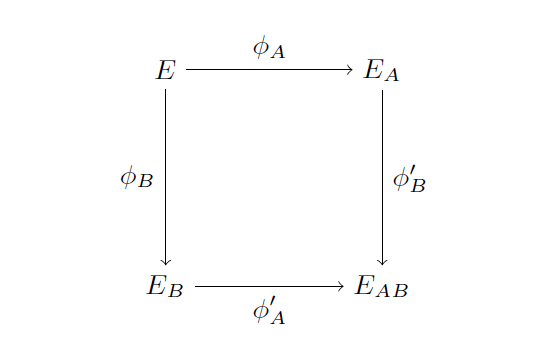
\includegraphics[width=0.5\textwidth]{razmena_kljuca.png}
	\caption{Protokol razmene ključa}
	\label{fig: razmena kljuca}
\end{figure}


\section{Napad umetanjem greške}

Pretrpostavimo da je napadnuti protokol otkriva $x$-koordinatu slike tačke pod tajnom izogenijom. Napad umetanjem greške cilja da natera implementaciju da kao rezultat da sliku slučajno odabrane tačke pod tajnom izogenijom. Ovo bi protivniku omogućilo da otkrije tajnu. Primetimo da ova izračunavanja ne uključuju $y$-koordinatu tačaka. 

Ako nam je daat kriva $E$ i tačka $P$, promena $x$-koordinate tačke $P$ rezultovaće drugom tačkom, $P_0$ na istoj krivoj. Ako nam je dato $x$ možemo da dobijemo $y$ rešavanjem kvadratne jednačine, koja u prostoru $\mathbb{F}_{p^2}$ uvek ima rešenje. Konkretno, svako $x \in \mathbb{F}_{p^2}$ odgovara tački na krivoj $E$ ili na krivoj $E'$, koja predstavlja njen kvadratni obrt. U najefikasnijim implementacijama kriptografskih sistema do sada, izračunavanja ne razlikuju krive $E$ i $E'$ tako da će izogenija biti izračunata tačno za svako $x \in \mathbb{F}_{p^2}$. 


\subsection{Dobijanje izogenije iz slike slučajno odabrane tačke}

Neka je $E/\mathbb{F}_{p^2}$ supersingularna eliptička kriva gde je  $p = l^{e_A}_{A} \cdot l^{e_B}_{B} \cdot f \pm 1$. Zatim sa tačkama ($P_A$, $Q_A$), ($P_B$, $Q_B$) i
($P_C$, $Q_C$) koje su generatori redom za $E[l^{e_A}_{A}]$, $E[l^{e_B}_{B}]$ i $E[f]$, slučajno odabrana tačka $X \in E(\mathbb{F_{p^2}})$ ima oblik

$$X = [u]P_A + [v]Q_A + [w]P_B + [x]Q_B + [y]P_C + [z]Q_C$$

\noindent za neke $u, v, w, x, y, z \in \mathbb{Z}$

Sad pretpostavimo da nam je data slika tačke $X$ pod izogenijom $\phi_A$, onda ćemo pokazati kako neko može da iskoristi $\phi_A(X)$ da dobije $\phi_A$. Pošto je $\phi_A$ homomorfizam grupe i znamo da $X$ može biti izraženo linearnom kombinacijom  $P_A$, $Q_A$, $P_B$, $Q_B$, $P_C$ i $Q_C$ imamo sledeći izraz

$$\phi_A(X) = \phi_A([u]P_A + [v]Q_A + [w]P_B + [x]Q_B + [y]P_C + [z]Q_C) $$
$$= [u]\phi_A(P_A) + [v]\phi_A(Q_A) + [w]\phi_A(P_B) $$
$$+ [x]\phi_A(Q_B) + [y]\phi_A(P_C) + [z]\phi_A(Q_C)$$


\noindent Sada nam je cilj da izolujemo linearnu kombinaciju $ \phi_A(P_A)$ i  $ \phi_A(Q_A)$. Do kraja izvodimo operaciju:

$$[l^{e_B}_{B} \cdot f]\phi_A(X) = [l^{e_B}_{B} \cdot f] ([u]\phi_A(P_A) + [v]\phi_A(Q_A))$$
$$= [u']\phi_A(P_A) + [v']\phi_A(Q_A)$$

Jednom kad dobijemo $ [u']\phi_A(P_A) + [v']\phi_A(Q_A)$, podgrupa generisana do sada će pomoći u konstruisanju izogenije $\phi_A$.


\textbf{Lema 1.} Neka je $E_1$ supersingularna eliptička kriva u $\mathbb{F}_{p^2}$, gde je $p = l^{e_A}_{A} \cdot l^{e_B}_{B} \cdot f \pm 1$. Pretpostavimo da je $\phi : E_1 \longrightarrow E_2$ izogenija stepena $l_A^{e_A}$ i  neka su $\{P, Q\}$ generatori za $E_1[l_A^{e_A}]$. Tada za bilo koje $X \in E[l_A^{e_A}]$ definiši $\psi : E_2 \longrightarrow E'$ takvo da je $ker \psi = \langle \phi(X) \rangle$, onda postoji $\theta: E' \longrightarrow E_1$ koje je stepena $l_A^t$, tako da je $t \leq e_A$, takvo da je 

$$\widehat{\phi} = \theta \circ \psi$$.  

Lema nam govori da ako nam je data slika tačke na krivoj $E_1[l^{e_A}_A]$ u izogeniji $\phi$, onda možemo da pronađemo izogeniju $\psi$ koja je približna izogeniji $\phi$. Kako bismo dobili $\psi$ prvo moramo da otkrijemo $\theta$. Ako je $t$ dovoljno malo, onda možemo dobiti $\theta$ grubom silom. U većini slučajeva $t$ jeste dovoljno malo. U nastavku je dat algoritam za dobijanje izogenije za slučajno odabranu tačku.


\begin{algorithm}
	\label{alg: napad greskom}
	\SetKwInOut{Input}{Data}
	\SetKwInOut{Output}{Output}
	
	\Input{$\phi(X)$}
	\Output{$\widehat{\phi}$}

	Postavi $\lambda \longleftarrow l_B^{e_B} \cdot f$ \;
	Postavi $T \longleftarrow [\lambda]\phi(X)$ \;
	Postavi $\psi: E_2 \longrightarrow E'$ kao izogeniju sa jezgrom $T$\;
	\eIf{ $ord(T) = l_A^{e_A}$}
		{
			return $\psi$
		}
		{
			Gruba sila za računanje $\theta$
		}
	return $\theta \circ \psi$
	\caption{Dobijanje izogenije nakon napada umetanjem greške}
\end{algorithm}


\subsection{Izvodljivost napada na protokol razmene ključeva}

Razmotrimo protokol razmene ključa opisanog u \ref{sec: razmena kljuca}. Pretpostavimo da protivnik pokušava da sazna Alisinu tajnu izogeniju i ima mogućnost da izazove grešku u ALisinom računu. Nakon računanja sa greškom, Alisa objavljuje ključ $(E_A; \phi_A(X), \phi_A(Q_B))$. Protivnik će onda biti u mogučnosti da otkrije $\phi_A$ pomoću Algoritma \ref{alg: napad greskom}.
\\
\\
Pretpostavimo da jedna strana koristi statički ključ u protokolu razmene ključeva. Protivnik bi bio u mogućnosti da otkrije tajnu izogeniju ako se statički javni ključ preračunava za svaku razmenu. Ipak, to nije verovatno da se desi jer se $\phi_A(P_B)$ i $\phi_A(Q_B)$ fiksiraju u programu (engl. hardcode) zbog efikasnosti. 
Sada pretpostavimo da protivnik napada protokol razmene ključa sa kratkotrajnim ključevima. Ako tajne nisu autentifikovane, protivnik je u mogućnosti da izračuna $\phi_A(P_B)$ i pošalje to umesto $\phi_A(X)$. Na ovaj način, obe strane mogu izvesti istu deljenu tajnu. Pošto se otkrivanje $\phi_A$ pomoću  $\phi_A(X)$ može izvesti efikasno i računanje  $\phi_A(P_B)$ je egikasno, izvođenje zamene pre nego što istekne vreme za konekciju je veoma izvodljivo. Ipak, treba primetiti da je, ako tajne nisu autentifikovane, bolje kotistiti napad ‚‚čovek u sredini'' (engl. man-in-the-middle attack).

\end{document}